%  !TeX  root  =  user_guide.tex

\section{Модуль интерполяции}

% when the revision of a section has been finalized,
% comment out the following line:
%\updatedisclaimer

Модуль интерполяции может использоваться для интерполяции точечного векторного слоя
методом триангуляции (TIN~--- Triangular Irregular
Network) или обратного взвешивания расстояний (IDW~--- Inverse Distance
Weighted). Данная операция довольно несложная и основывается на интуитивно понятном графическом
интерфейсе для создания интерполированных растровых слоев (cм. Рисунок~
\ref{fig:interpolation_dialog}). Модуль требует наличия следующих
параметров для выполнения:

\begin{itemize}[label=--]
\item \textbf{Исходный векторный слой}: Выберите исходный точечный
векторый слой из списка загруженых точечных слоев. Если выбраны
несколько слоев, для интерполяции используются данные всех слоев.
Примечание: существует возможность вставки линий или полигонов в
качестве ограничений для триангуляции; для этого необходимо выбрать
<<Линии структуры>> или <<Линии разбивки>> в выпадающем меню
\dropmenuopt{Тип}.
\item \textbf{Атрибут интерполяции}: Выберите необходимый атрибут
для интерполяции или установите флаг
\checkbox{Использовать для интерполяции Z-координату} для того, чтобы
задействовать значения Z, хранимые в слоях.
\item \textbf{Метод интерполяции}: Выберите метод интерполяции. Это
может быть либо \\
\selectstring{{}Триангуляция (TIN)}{\ldots} или же \\
\selectstring{{}Обратное взвешивание расстояний (IDW)}{\ldots}.
\item \textbf{Количество столбцов/строк}: Выберите количество строк и
столбцов в результирующем растровом файле.
\item \textbf{Файл вывода}: Выберите название для выходного растрового
файла.
\end{itemize}

\begin{figure}[ht]
   \centering
   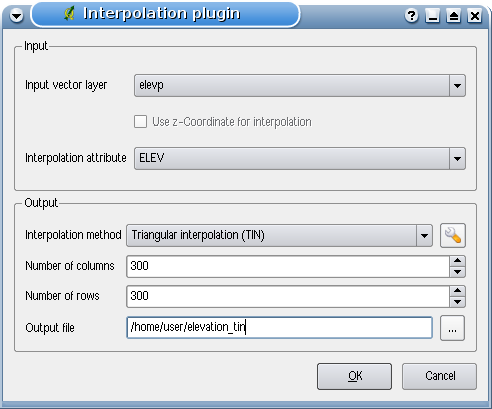
\includegraphics[clip=true, width=14cm]{interpolate_dialog}
   \caption{Модуль интерполяции \wincaption}\label{fig:interpolation_dialog}
\end{figure}

\minisec{Использование модуля}\label{interpolation_usage}

\begin{enumerate}
  \item Запустить QGIS и загрузить точечный векторый слой (к примеру,
  \filename{elevp.csv}).
  \item Активировать модуль интерполяции через <<Управление модулями>>
  (см. Раздел~\ref{sec:load_core_plugin}), а затем нажмите по иконке
  \toolbtntwo{interpolation}{Интерполяция}, которая появится на панели
  инструментов QGIS. Откроется диалоговое окно модуля интерполяции, как
  показано на рисунке~\ref{fig:interpolation_dialog}.
  \item Выбрать исходный слой (к примеру, \selectstring{{}elevp}{\ldots})
  и колонку (к примеру, \filename{ELEV}) для интерполяции.
  \item Выбрать метод интеполяции (например,
  \selectstring{{}Триангуляция}{\ldots}) и установить <<Разрешение по Х>>
  и <<Разрешение по Y>> равным 5000, а также задать название растрового
  файла вывода (например, \filename{elevation\_tin}).
  \item Нажать \button{Ok}.
  \item В данном примере дважды кликнуть \filename{elevation\_tin}
  в списке слоев, чтобы открыть диалоговое окно свойств растрового слоя
  и выбрать \selectstring{{}Псевдоцвет}{\ldots} в качестве Цветовой
  карты на закладке \tab{Символика}. Или же определить новую таблицу
  раскраски, как описано в разделе~\ref{label_rasterprop}.
\end{enumerate}

На рисунке~\ref{fig:interpolation_idw} показан результат интерполяции
TIN с разрешением 998~колонок на 812~строк (5~км) для файла
\filename{elevp.csv} с применением цветовой карты <<Псевдоцвет>>. Сама
обработка заняла несколько минут. Созданный растр покрывает северный район Аляски.

\begin{figure}[ht]
   \centering
   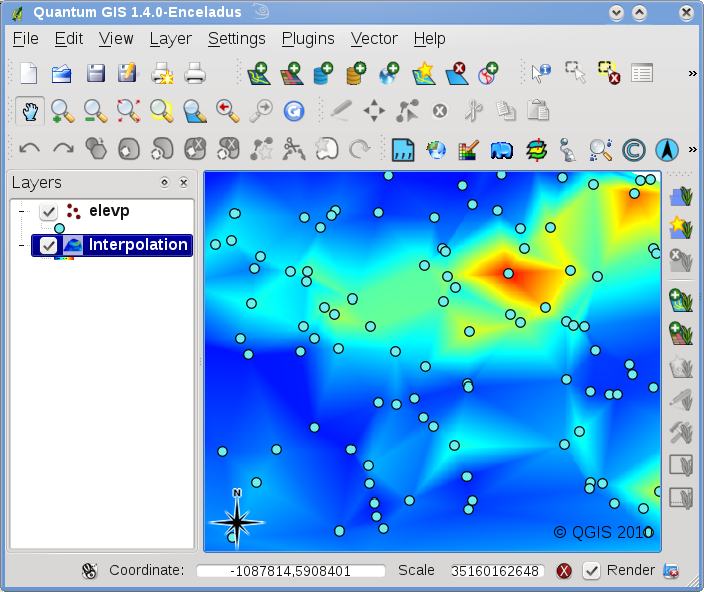
\includegraphics[clip=true, width=10cm]{interpolate_tin}
   \caption{Интерполяция высотных данных методом TIN \wincaption}\label{fig:interpolation_idw}
\end{figure}

\FloatBarrier
